\subsection*{e. Disminuir 8\% los precios de los productos de la categoría Furniture cuyo precio sea de \$600 a \$900. Aumentar en un 5\% los precios de los productos de la categoría Technology y subcategoría Machines.}

Primero filtramos los productos de la categoría \textit{Furniture} que cumplen con el rango de precios (600 a 900) mediante una selección, y guardamos el resultado como \textit{furn\_old}. Hacemos lo mismo para filtrar los productos de \textit{Technology} y subcategoría \textit{Machines}, guardándolos en \textit{tech\_old}, estos dos últimos serán los que vamos a eliminar. A continuación, utilizamos la proyección para generar las tuplas actualizadas. Para los muebles, aplicamos un descuento del 8\% multiplicando el \textit{price} por $0.92$, asignándolo al mismo nombre en \textit{furn\_new}. Para la tecnología, aplicamos el aumento del 5\% multiplicando por $1.05$ en \textit{tech\_new}. Finalmente, llevamos a cabo el mantenimiento en la relación general \textit{products}: borramos (restamos) las tuplas originales que apartamos, y unimos (insertamos) los subconjuntos nuevos calculados.

Expresión:
\begin{equation}
\begin{split}
\text{furn\_old} &= \sigma_{category = \text{'Furniture'} \, \wedge \, price \ge 600 \, \wedge \, price \le 900}(products) \\
\text{tech\_old} &= \sigma_{category = \text{'Technology'} \, \wedge \, subcategory = \text{'Machines'}}(products) \\
\text{furn\_new} &= \pi_{productid,\, category,\, subcategory,\, price \cdot 0.92 \rightarrow price}(\text{furn\_old}) \\
\text{tech\_new} &= \pi_{productid,\, category,\, subcategory,\, price \cdot 1.05 \rightarrow price}(\text{tech\_old}) \\
\text{Resultado} &= (products - \text{furn\_old} - \text{tech\_old}) \cup \text{furn\_new} \cup \text{tech\_new}
\end{split}
\end{equation}

Resultados obtenidos:

\begin{figure}[h!]
\centering
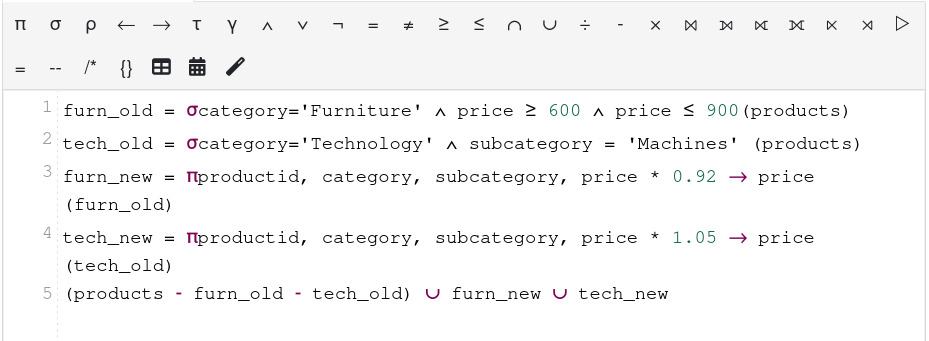
\includegraphics[width=0.8\textwidth]{imagenes/3e(1).png}
\caption{Consulta 3e.}
\end{figure}

\begin{figure}[h!]
\centering
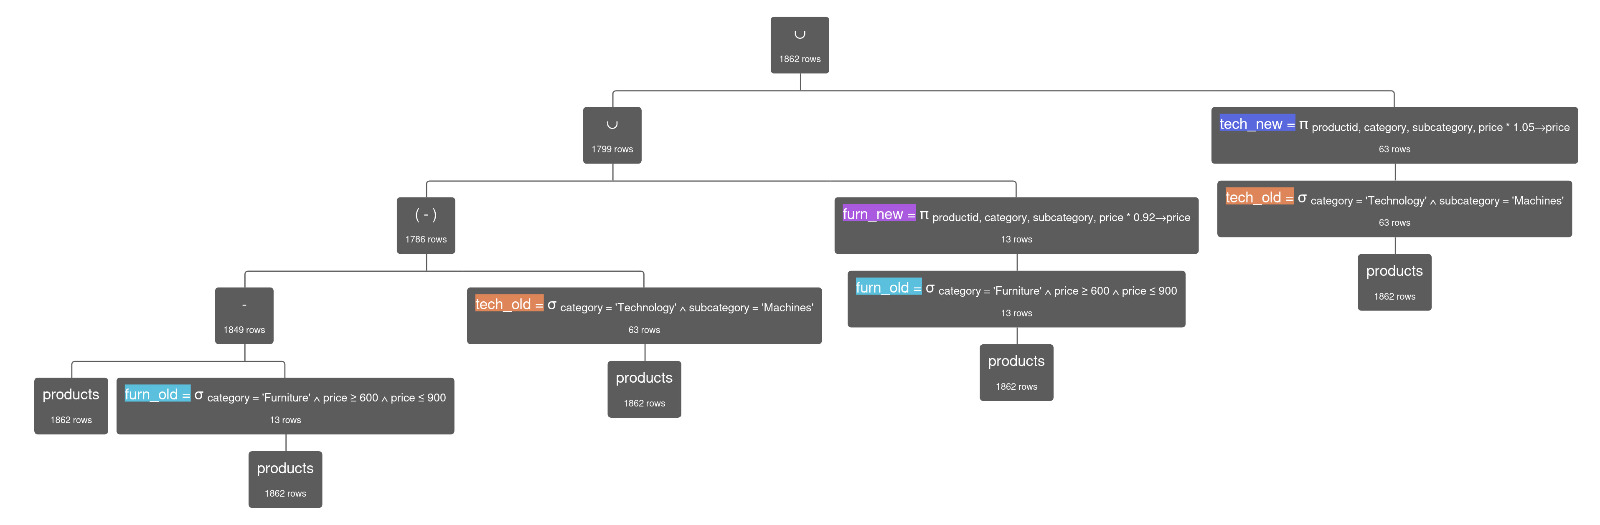
\includegraphics[width=0.8\textwidth]{imagenes/3e(2).png}
\caption{Árbol de consulta 3e.}
\end{figure}

\begin{figure}[h!]
\centering
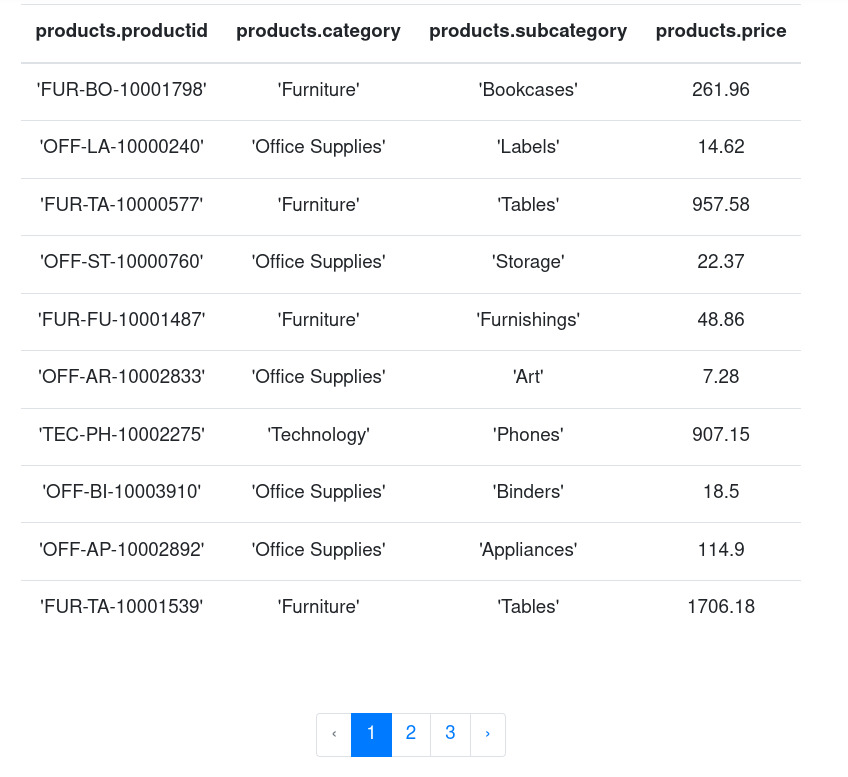
\includegraphics[width=0.6\textwidth]{imagenes/3e(3).png}
\caption{Resultado de consulta 3e.}
\end{figure}
